\section{Satz (Parallelogrammgesetz)}
%
	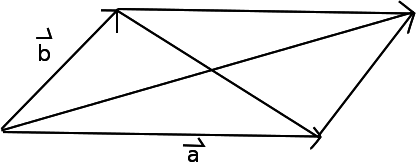
\includegraphics[width=0.45\textwidth]
	{mainmatter/chapter2/pics/para1.png}
%
$\left\Vert\vec{a} + \vec{b}\right\Vert + \left\Vert\vec{a} - \vec{b}\right\Vert^{2}$
$= 2\left\Vert\vec{a}\right\Vert^2 + 2\left\Vert\vec{b}\right\Vert^2$
%
%
%
\subsubsection{Beweis}
$<\vec{a} + \vec{b}, \vec{a} + \vec{b}> + <\vec{a} -\vec{b}, \vec{a} - \vec{b}>$
$= 2<\vec{a}, \vec{a}> + 2<\vec{b}, \vec{b}>$
%
%
%